\documentclass[twoside]{article}

\usepackage[dvipsnames]{xcolor}
\usepackage{tikz}
\usetikzlibrary{shapes,arrows}
\usepackage{caption} 
\usepackage[letterpaper]{geometry}
\usepackage{pdfpages}
\usepackage[normalem]{ulem}
\usepackage{wrapfig}
\usepackage{hyperref}
\usepackage{tcolorbox}
\usepackage{epigraph}

\newcommand{\mientrastanto}{``!`mientras tanto, los MAGOS DEL TIEMPO!''}

\hypersetup{
     colorlinks = true
}

\newcommand{\twsse}{\emph{Time Wizards: The Sober and Serious Edition}}
\newcommand{\tw}{\emph{Time Wizards}}
\newcommand{\sse}{\emph{Sober and Serious Edition}}
\newcommand{\rfe}{\emph{Revised First Edition}}
\newcommand{\vers}{$0.2.2 \beta$}

\tikzstyle{decision} = [diamond, draw, 
    text width=4.5em, text badly centered, node distance=3cm, inner sep=0pt]
\tikzstyle{block} = [rectangle, draw, 
    text width=5em, text centered, rounded corners, minimum height=4em]
\tikzstyle{line} = [draw, -latex']

\definecolor{anongreen}{HTML}{117743}
\newcommand{\anon}[1][]{{\color{anongreen} \textbf{Anonymous}#1}}
\newcommand{\namefag}[2][]{{\color{anongreen} \textbf{#2}#1}}

\newenvironment{examplebox}[1]{\begin{tcolorbox}[colback=green!5!white,colframe=green!75!black,title={Example: #1}]}{\end{tcolorbox}\vspace{-30pt}}

\AtBeginDocument{\let\textlabel\label}

\begin{document}

\setcounter{page}{-3}

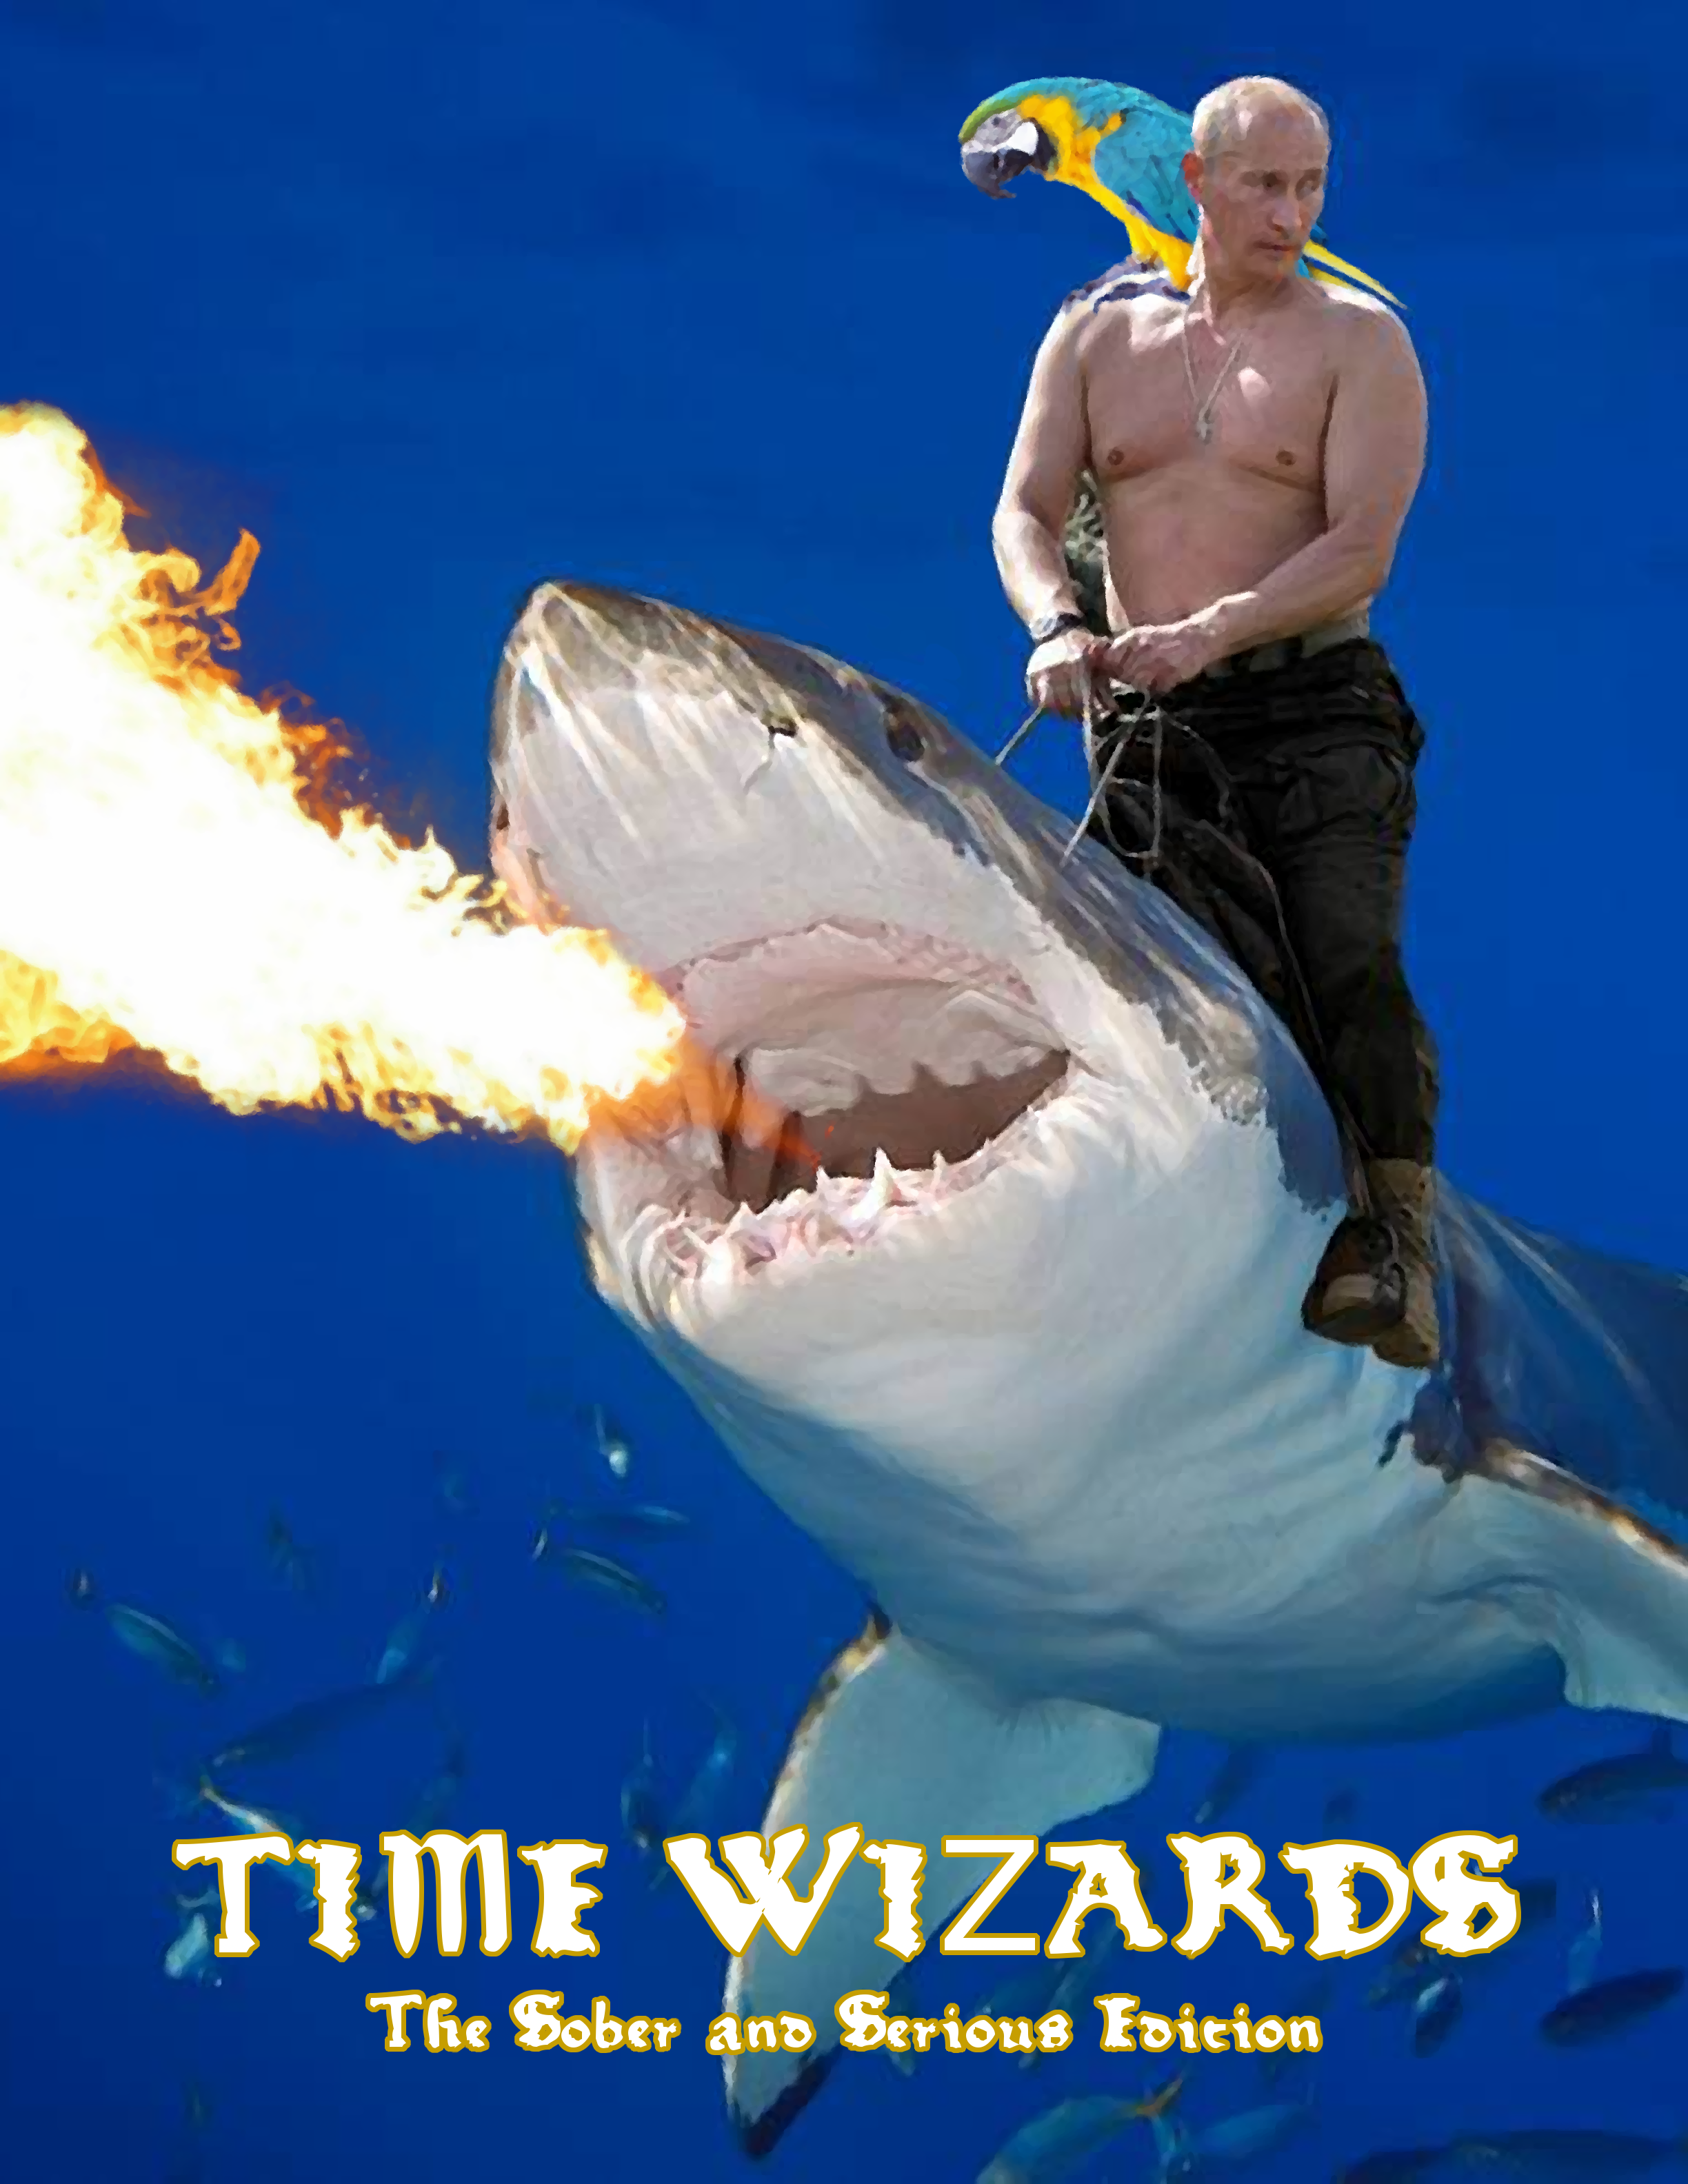
\includepdf[fitpaper]{cover}
\pagestyle{empty}
\cleardoublepage

\setcounter{tocdepth}{2}
\tableofcontents
\cleardoublepage

\pagestyle{plain}

\section{Introduction} \label{sec:intro}
\subsection{The Game of \tw{}} \label{ssec:gameintro}
\epigraph{\textbf{Why should you play \tw{}?} You should not play \tw{}.}
   {\emph{Time Wizards: Classic Edition}}
\tw{} is equal parts tabletop game and improv comedy routine, in which players use a ridiculous
mockery of logic and reality-bending everyday tasks to accomplish an objective set by the Time
Master (TM). The success or failure of any individual task is determined by dice; the scope and
nature of the tasks are determined largely only by player imagination.

\tw{} is not a game where dice determine outcomes; the dice only determine who determines the
result. Rather than picking out the best numbers and most useful rules, \tw{} players should
try and have a good grasp of lateral thinking, some understanding of the rules of logic, and
access to a thesaurus. Knowing what to say and how to say it will do far more for you than
probability calculations.

\tw{} is a short game: a typical session might last an hour, while a long session would run two.
It's not something you get together specifically to play, but something played to pass the time
while your usual GM naps, while you're waiting for the pizza to arrive, or after the main event
is over and a few people are still lingering around their chairs.

\tw{} is not about the destination: it's pretty easy to get whatever the players want done, done
eventually. The appeal isn't in accomplishing what you set out to do, it's in the ridiculous
complications that are inevitably introduced by the whims of the dice gods and the sheer chaos
a group of Time Wizards leave in their wake. A simple trip to the local florist may well end in
the party clinging desperately to a rampaging Hypercorgi as it gnaws curiously on Big Ben.

\subsection{About This Document} \label{ssec:rulesintro}
This document details the rules of what we call \twsse{}, a game for serious individuals
with serious lives. At least, by the standards of \tw{} players, which is sort of like saying
``a particularly Chaotic sort of paladin'' or ``a very healthy lich''. As the name might 
(somewhat jokingly) suggest, \sse{} is an attempt at producing a game with similar potential for
shenanigans as traditional \tw{} while being more accessible to a general tabletop audience.

This ``edition'' is very much a work in progress, and any playtest information you have is very
welcome; \namefag{Time Wizard Archibald}, the main author of this document, can be contacted with
any feedback at \verb|archie.m.vist@gmail.com|. The latest version of the document is available
on GitHub at \url{https://github.com/archie-m-vist/time-wizards/releases}.

For reference, this is version \vers{} of \twsse. This version introduces time paradox
mechanics, reorganises several sections, and introduces a series of play examples; in addition,
we have split the comparisons to previous versions of \tw{} into its own document.

\section{Setting Up} \label{sec:setup}
First, it is absolutely pivotal to begin a game of \tw{}, no matter what edition, with a loud
and joyous cry of \mientrastanto. If you can't even pretend to speak Spanish, any local
equivalent of ``Meanwhile, the Time Wizards!'' is acceptable. Before beginning play, also
determine who will be acting as players, controlling a Time Wizard within the game world, and
who will be the Time Master. The Time Master, also referred to as the TM, is responsible for
suggesting the powers of the Time Wizards to each player, developing the scenario and objective
that the Time Wizards are presented with, and rolling dice to oppose the Time Wizards' attempts
to use their powers.

\begin{wrapfigure}{o}{0.5\textwidth}
   \vspace{-10pt}
   \begin{examplebox}{Beginning Play}
      Nicol, Connie, Urist, and Hassan have gathered to play a friendly game of \tw{}. After a
      call of \mientrastanto{} to declare the session open, Nicol, as the most experienced GM of
      the group, volunteers as Time Master.

      Since they're all still inexperienced with \tw{}, they decide not to adopt any Doctrines
      for this session.
   \end{examplebox}
   \vspace{15pt}
\end{wrapfigure}

Typically, the Time Master will be a player familiar with the rules (such as they are) of \tw{},
or someone with experience running games. Keep in mind, though, that players need to get
experience somehow and your TM probably wants a chance to play as well, so once you've all played
a few games, try switching up who is the TM and who is playing.

Conventional \tw{} also suggests the addition of one silly house rule, referred to as a Doctrine,
by each player. \twsse{} does not officially require Doctrines, but their addition can bring
excellent further antics with an experienced groups. Doctrines can be strictly mechanical
(``reroll all threes''), strictly social (``every time you say sentence with three or more Qs
in it, take a drink''), or a hybrid of the two (``every time a player swears, 1d6 sheep appear
surrounding their character''). We suggest that inexperienced

\subsection{Character Creation} \label{ssec:creation}
Each player in a game of \tw{} controls a single Time Wizard: mighty masters of time and space
who warp reality to their will in both highly-specific yet completely open-ended ways. Prior to
their sudden, unexpected ascendancy to Time Wizardhood, a Time Wizard is an individual going
about an ordinary day who is suddenly and instantaneously imbued with mighty eldritch powers,
based on some of the last things they did as a mortal man.

\tw{} does not use elaborate character sheets or blocks of numbers. Each Time Wizard has five
powers, which are chosen by the player from a list given by the Time Master, and two numerical
statistics (one of which is simply ten minus the other). There are two types of character
resources determined by these values, Posits and Power, both of which are spent in order to use
Time Wizard powers. These are the extent to which a \tw{} player has to keep track of anything.

\subsubsection{Determine Powers} \label{ssec:get-powers}
First, when creating your Time Wizard, determine what your character's mortal life was like;
this lets you give the TM ideas about what your character was doing. The TM then proceeds to
describe the events of your character's life through sets of phrases in the general form
``verb the noun'': that is, performing some action on some object.

\begin{wrapfigure}{o}{0.5\textwidth}
   \vspace{-25pt}
   \begin{examplebox}{Determining Powers}
      Connie decides that her character was a bricklayer prior to becoming a Time Wizard. Nicol
      then chooses a time and date, in this case Wednesday at 4:15 in the Afternoon, at which
      point he begins listing abilities.

      Nicol decides that each set of powers he provides will have six powers in it: his first
      set of powers for Connie is ``scale the scaffolding'', ``pour the mortar'', ``hear the
      foreman'', ``fasten the brick'', ``lower the trowel'', and ``bite the sandwich''. He
      then gives a set of six other powers to Urist and to Hassan, in order of their seating.

      Reaching Connie again, he provides six more powers: ``traverse the ladder'', ``reach the
      ground'', ``end the shift'', ``find the bus'', ``take the ride'', and ``call the house''.

      Connie thinks these sets are fine, and chooses five powers from them: ``pour the mortar'',
      ``bite the sandwich'', ``reach the ground'', ``fasten the brick'', and ``end the shift''.
   \end{examplebox}
\end{wrapfigure}

There is no set size for the number of phrases provided by the TM to a player, but each set must
contain at least five powers. We recommend that each set given to each player is of the same
size, in order to give each player equal opportunity to choose their powers. Players may select
five powers from the last two sets provided to them by the TM: they can reject the older set for
a new one, but cannot revisit it once it has been dismissed.

What a character does in their pre-Time Wizard life is entirely up to the player; however, the
TM is under no obligation to make exciting characters have exciting powers: they must be
going about an ordinary day, no matter how extraordinary the character may be. Even if someone
were could be the ruler of all known space, the day they awakened to Time Wizard powers would be
the day they went to a wine tasting and caught up on paperwork. It is for this reason that
Theodore Roosevelt cannot become a Time Wizard. Theodore Roosevelt does not need to become a
Time Wizard.

\subsubsection{Determine Characteristics} \label{ssec:get-characteristics}
With your character's five powers chosen, you must then allocate your Time Wizard's
characteristics. Time Wizards are rather simple entities, with two characteristics: Will,
representing the Time Wizard's mental fortitude, and a second stat which represents their
ability to understand and use their Time Wizard powers. The name of this stat is chosen by each
Time Wizard based on something in their past life; for instance, a stage magician may attribute
their newfound powers to their Showmanship, while a bodybuilder might attribute it to their
Musculature. For consistency, we will call this a Core Attribute; it can be any attribute of the
character, usually something they see as a definitive aspect of themselves.

\begin{wraptable}{o}{0.5\textwidth}
   \caption{CA and Will Values}
   \label{tab:cawill}

   \begin{tabular}{cc|ccc}
   \textbf{CA} & \textbf{Will} & Posits & Power & Dice Cap\\ \hline
      1 & 9 &  5 & 45 &  3\\
      2 & 8 &  8 & 40 &  4\\
      3 & 7 & 11 & 35 &  5\\
      4 & 6 & 14 & 30 &  6\\
      5 & 5 & 17 & 25 &  7\\
      6 & 4 & 20 & 20 &  8\\
      7 & 3 & 23 & 15 &  9\\
      8 & 2 & 26 & 10 & 10\\
      9 & 1 & 29 &  5 & 11
   \end{tabular}
\end{wraptable}

A Time Wizard's two characteristics must sum to 10: if Captain Ahab the Time Wizard has 7 Desire
To Slay The Whale, he must then have 3 Will. Increasing one decreases the other, so it's only
really necessary to track one, but having both written out is an easy reminder of your Time
Wizard's abilities.

Time Wizards have access to two pools of power: their Power pool, which is determined by Will,
and their Posits, which are determined by their Core Attribute. A time wizard has a maximum of
five times their Will in Power, and has three times their Core Attribute plus two in Posits.
A ``balanced'' Time Wizard has 5 Will and 5 Core Attribute, for a total of 25 Power and 17
Posits. A full listing of Time Wizard attribute choices and their results is given in
\hyperref[tab:cawill]{Table \ref*{tab:cawill}: CA and Will Values}.

To ``Posit'' means to put forward a logical proposition, and is also a homophone for ``pause
it'' if you have the right accent. This suggests the function of a Posit: to declare a Time
Moment and to expand the function of your Time Wizard powers beyond their mundane trappings.
Declaring a Time Moment, dilating time, and making outlandish prepositions for your Time Wizard
powers all require at least one Posit be spent.

\begin{wrapfigure}{o}{0.5\textwidth}
   \vspace{-10pt}
   \begin{examplebox}{Determining Characteristics}
      Hassan wants his Time Wizard, Thursday at 11:05 in the Morning, to be able to throw more
      dice, and thus win against Nicol more often, but he doesn't want to run out of Power
      either. He settles for 4 Will and 6 Core Attribute: he can throw $6+2=8$ dice, and has
      $5\cdot 4=20$ Power and $2+3\cdot 6=20$ Posits.
   \end{examplebox}
   \vspace{20pt}
\end{wrapfigure}

Power is more straightforward: you can spend a point of power to either add a single d6 to your
roll to activate a power, or to increase the breadth of the power you are using. The maximum
number of dice you can roll is given in the nearby table under Dice Cap; power to breadth
conversion is up to the TM, but general suggestions are given in
\hyperref[tab:powersize]{Table \ref*{tab:powersize}: Power to Size Guidelines}.

Generally, Will increases the amount of times you can use your powers by means of increasing
your maximum Power pool, while Core Attribute makes each use of your power more successful and
with greater influence. If you're uncertain as to which build to take, we recommend either 5
of both or 4 of one stat and 6 of the other.

With your characteristics and powers determined, your Time Wizard is ready to play!

\subsection{The Scenario} \label{ssec:scenario}
When every party member has finished character creation, the Time Master outlines the situation
and objective of the party. \twsse{}, like all forms of \tw{}, is not designed for long
campaigns\footnote{But if you run one, storytime that shit.}; generally, you'll be playing for
an hour or so after another game, or to kill time during the day. It's highly recommended to
have a straightforward objective for the players to focus their energies on, or else the game
drags for lack of purpose.

A good scenario can be anything from ``Liberate the world's supply of croissants'' to ``Kill
Hitler'' to ``Steal the Hope Diamond (to pay your rent)''. (These are all from actual games of
\tw{} I have played or TM'd: the first and third in \rfe{}, the second being the inaugural game
of \sse{}.) Any task that isn't trivially simple can be complicated by the sheer chaos that a
group of Time Wizards will inevitably bring to any goal; the fun of \tw{} isn't achieving the
objective, it's everything that happens along the way.

\section{Time Moments} \label{sec:time-moment}
With player characters and a scenario, it's time to play the game. The Time Wizards can bumble
around in an active universe and try and do things like ordinary people; there aren't really
rules for this right now, so it's largely to the TM's discretion how events occur in normal time
(if they really matter at all). Essentially, normal-time gameplay is made up of two things:
waiting for a Time Moment, and the immediate aftermath of a Time Moment.

A Time Moment is a frozen instant in time, during which the Time Wizards may use their powers.
Movement and direct action are impossible; the only thing that can happen during a Time Moment
is the use of Time Wizard powers. \hyperref[fig:timemoment]{Figure \ref*{fig:timemoment}: Flow
of a Time Moment} shows the general structure of a Time Moment in \twsse{}.

The colours in the figure indicate a grouping according to the section in the rules: red is
covered under \nameref{ssec:begin-moment}, yellow under \nameref{ssec:power-declaration}, green
under \nameref{ssec:roll-phase}, cyan under \nameref{ssec:resolve-power}, blue under
\nameref{ssec:time-paradox}, purple under \nameref{ssec:time-dilation}, and
\nameref{ssec:end-moment}.

\begin{figure}
   \caption{Flow of a Time Moment}
   \label{fig:timemoment}

   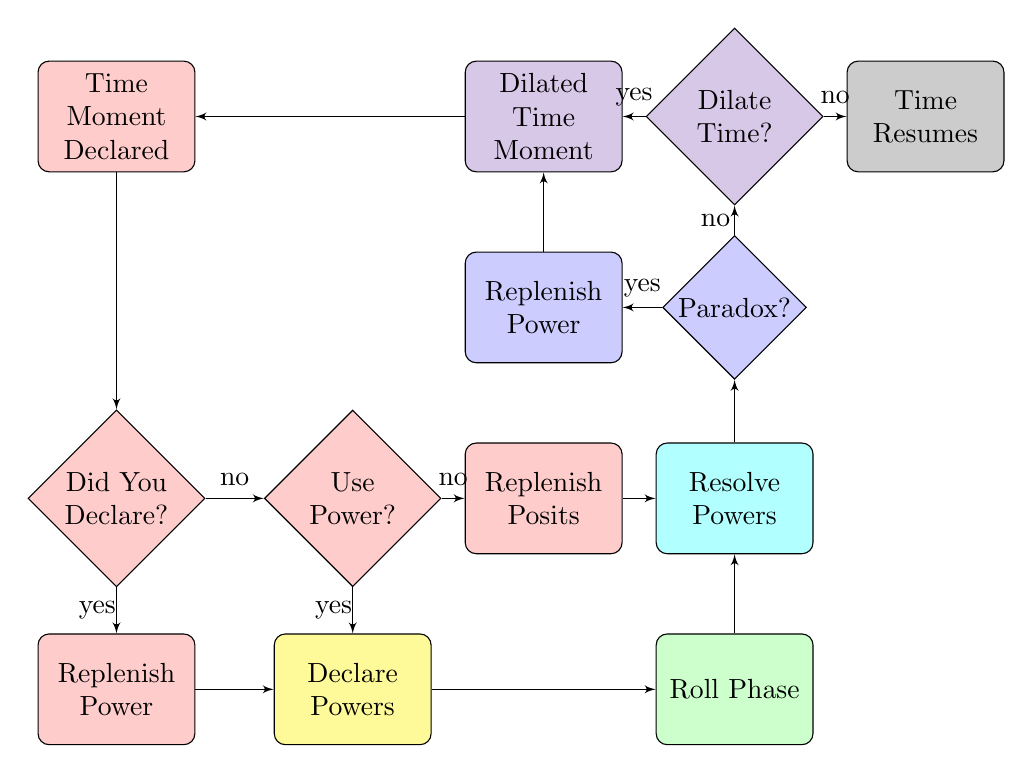
\begin{tikzpicture}
      \node [block, fill=red!20] (init) {Time Moment Declared};
      \node [decision, below of=init, fill=red!20, node distance=0.4\textwidth] (determine)
         {Did You Declare?};
      \node [decision, right of=determine, fill=red!20] (decide) {Use Power?};
      \node [block, right of=decide, node distance=0.2\textwidth, fill=red!20] (posits)
         {Replenish Posits};
      \node [block, below of=determine, node distance=0.2\textwidth, fill=red!20] (power)
         {Replenish Power};
      \node [block, below of=decide, node distance=0.2\textwidth, fill=yellow!40] (declare)
         {Declare Powers};
      \node [block, right of=declare, node distance=0.4\textwidth, fill=green!20] (roll)
         {Roll Phase};
      \node [block, above of=roll, node distance=0.2\textwidth, fill=Cyan!30] (resolve)
         {Resolve Powers};
      \node [decision, above of=resolve, node distance=0.2\textwidth, fill=blue!20] (paradox)
         {Paradox?};
      \node [block, left of=paradox, node distance=0.2\textwidth, fill=blue!20] (parapower)
         {Replenish Power};
      \node [decision, above of=paradox, node distance=0.2\textwidth, fill=RoyalPurple!20]
         (dilate) {Dilate Time?};
      \node [block, right of=dilate, node distance=0.2\textwidth, fill=black!20] (done)
         {Time Resumes};
      \node [block, left of=dilate, node distance=0.2\textwidth, fill=RoyalPurple!20] (new)
         {Dilated Time Moment};

      \path [line] (init) -> (determine);
      \path [line] (determine) ->
         node [left of=start, node distance=0.02\textwidth] {yes} (power);
      \path [line] (determine) ->
         node [above of=start, node distance=0.02\textwidth] {no} (decide);
      \path [line] (decide) ->
         node [left of=start, node distance=0.02\textwidth] {yes} (declare);
      \path [line] (decide) -> node [above of=start, node distance=0.02\textwidth] {no} (posits);
      \path [line] (power) -> (declare);
      \path [line] (posits) -> (resolve);
      \path [line] (declare) -> (roll);
      \path [line] (roll) -> (resolve);
      \path [line] (resolve) -> (paradox);
      \path [line] (paradox) -> node [left of=start, node distance=0.02\textwidth] {no} (dilate);
      \path [line] (paradox) -> node [above of=start, node distance=0.02\textwidth] {yes}
         (parapower);
      \path [line] (dilate) -> node [above of=start, node distance=0.02\textwidth] {yes} (new);
      \path [line] (dilate) -> node [above of=start, node distance=0.02\textwidth] {no} (done);)
      \path [line] (parapower) -> (new);
      \path [line] (new) -> (init);
   \end{tikzpicture}
\end{figure}

\subsection{Beginning a Time Moment} \label{ssec:begin-moment}
A Time Wizard may declare a Time Moment at any time for the cost of one Posit; if they have no
Posits available, they cannot declare a Time Moment, and are helpless save for the intervention
of their fellow Time Wizards. As soon as the Time Moment is declared, time freezes and the
Time Wizards step away from reality, ready to work their havoc upon it.

\begin{wrapfigure}{o}{0.5\textwidth}
   \vspace{-10pt}
   \begin{examplebox}{Beginning of a Time Moment}
      Urist spends a Posit to declare a Time Moment, and regains 11 power out of his max of 35.
      Connie declines to participate while Hassan decides to use a power: with two powers being
      used, Connie regains two Posits.
   \end{examplebox}
   \vspace{20pt}
\end{wrapfigure}

The Time Wizard who declares the Time Moment regains one third of their maximum Power, rounded
down, upon declaration; however, they must declare a power to use during this Time Moment, which
means that declaring a Time Moment purely to recharge Power can be a dangerous proposition: as
the player must roll against the TM, this can reduce the amount of power regained unless the
player is willing to gamble on the TM's imagination and what can happen to their Time Wizard
after a low-power Roll.

Time Wizards who did not declare the Time Moment can choose as to whether or not they
participate. Those who do move on to declaring powers; those who do not regain one Posit for
each power being used in this Time Moment, including the power used by the declarer.

\subsection{Power Declaration} \label{ssec:power-declaration}
The Time Wizards who decide to participate in a Time Moment must then declare which of their
five powers they intend to use, and the amount of their Power they intend to use. One point of
Power adds one die to the amount rolled, or increases the size of the effect. Effect sizes are
given in \hyperref[tab:powersize]{Table \ref*{tab:powersize}: Power to Size Guidelines}; it'
good to ask the TM for specific sizes of objects to determine the Power that needs to be spent
to influence it.

\begin{wrapfigure}{o}{0.5\textwidth}
   \begin{examplebox}{Declaring Powers}
      Nicol decides on an Order Rating of 4.

      Urist announces that he will ``swing the club'' over the range of a city block, and will
      roll all five of his dice: this costs him 8 Power.

      Hassan will ``welcome the customer'' on a single other individual, and will roll six dice:
      this costs him 7 Power.
   \end{examplebox}
   \vspace{25pt}
\end{wrapfigure}

The reason that Power amount is declared prior to dice being rolled is to prevent players
changing their range or dice count in response to knowledge of the Time Master, and to place a
limit on the range that the Time Master can operate on if they win.

\begin{wraptable}{o}{0.5\textwidth}
   \caption{Power to Size Guidelines}
   \label{tab:powersize}

   \begin{tabular}{c|c}
      \textbf{Power Spent} & {Size Limit}\\ \hline
      0 & The power's user only\\
      1 & A person\\
      2 & A house or building\\
      3 & A city block\\
      4 & A small town\\
      5 & A large city\\
      6 & A small country\\
      7 & A continent\\
      8 & A planet\\
      9 & A star system\\
      10 & A galaxy\\
      11 & The entire universe
   \end{tabular}
   \vspace{-24pt}
\end{wraptable}

Further Power-to-area tiers can be added at the TM's discretion. So long as the Time Wizard has
the power in their pool, there is no limiting factor for spending it on area of
effect.\footnote{Yes, we know it's actually a volume of effect.} Suggested values for 12 Power
include the entire multiverse, if such a thing is pertinent to your game, or a cluster of
related universes if the multiverse is truly large. Another use for high Power would be to
interfere with other games of \tw{} occurring in the same area, so long as your Time Masters
have an understanding.

When using Power to increase the number of dice rolled when activating a power, note that the
number of added dice cannot exceed the Time Wizard's Core Attribute score. The maximum number
of dice a Time Wizard with a given attribute spread can roll is given under Section
\ref*{sec:setup}, in \hyperref[tab:cawill]{Table \ref*{tab:cawill}: CA and Will Values}.

\subsection{The Roll Phase} \label{ssec:roll-phase}
\begin{wrapfigure}{o}{0.5\textwidth}
   \vspace{-15pt}
   \begin{examplebox}{The Roll Phase}
      As Urist declared the Time Moment, he rolls first: he rolls a 6, a 4, two 3s, and a 2 for
      a total of 18. As the Order Rating is 4, Nicol rolls 4d6, and gets a 5, a 4, and two 1s
      for a total of 11. Urist wins the roll. Urist gets to resolve ``swing the club'', and
      gains a point of Wrath.

      Hassan rolls after Nicol: he gets two 4s, a 3, two 2s, and a 1 for a total of 12. Nicol
      again rolls 4d6, and gets a 6, two 5s, and a 3 for a total of 20. Nicol gets to resolve
      ``welcome the customer'', but Hassan does not gain any Wrath.
   \end{examplebox}
   \vspace{20pt}
\end{wrapfigure}

Once the amount of Power used by each Time Wizard is determined, each Time Wizard rolls their
chosen number of dice, beginning with the player who declared the Time Moment and moving through
the rest of the active Time Wizards in some order from there. (While the TM can decide this, we
suggest clockwise order or some other standard to keep things somewhat consistent.) These rolls
are opposed by another roll from the TM, based on the Order of the situation.

The more chaotic and disorderly a situation is, the more the Time Wizards thrive in it. If a
situation is already frantic and chaotic, the relative influence of the Time Wizards'
reality-breaking powers isn't as obvious, and the universe puts up less resistance. The amount
of resistance to Time Wizard interference exhibited by the environment is referred to as the
Order Rating, or simply Order; this is set by the TM, and changes based on the actions of the
players. Maintaining a low Order Rating allows Time Wizards to achieve more success for less
Power, but also places them at risk when time is in motion.

Normally, assuming there's no Wrath involved, the TM rolls 1d6 for each point of Order. The
winner of the roll is whichever player has a higher number; in the event of a tie, the winner
goes to whichever player rolled fewer dice. In the event that both of these are a tie, the
Time Wizard succeeds. When a Time Wizard succeeds, they get to choose how their power resolves
and they gain a point of Wrath; when a Time Wizard fails, the TM chooses how the power resolves.

\subsubsection{Wrath} \label{sssec:wrath}
Wrath is the representation of how much reality is sick of a given Time Wizard's shit. For
every successful roll against the TM, a Time Wizard gains a point of Wrath. When a Time Wizard
attempts to activate a power, the TM may use accumulated Wrath one of two ways: a single point
of Wrath will add one die to the roll against that power, or will increase the size of all dice
rolled against that power: a single point of Wrath will have the TM roll d8s, two will see
d10s, three will see d12s, and four will see d20s. This allows the TM to hijack particularly
useful Time Wizard powers and gain revenge on highly successful players even at low Order.

If Captain Ahab the Time Wizard were to ``hoist the rigging'' with an Order Rating of 2 and he
had accumulated five points of Wrath, the TM could spend three points to roll 4d8 instead of
2d6, greatly improving his odds of winning the roll. These three points are consumed regardless
of the outcome, leaving Captain Ahab with two points of Wrath (if he loses) or three points of
Wrath (the two remaining, plus the one gained by a successful roll).

\subsection{Resolving Powers} \label{ssec:resolve-power}
\begin{wrapfigure}{o}{0.5\textwidth}
   \vspace{-10pt}
   \begin{examplebox}{Power Resolution}
      Urist decides to use his power ``swing the club'' over the size of a city block, and beats
      Nicol during the roll phase. He proposes the following chain of logic:

      \textbf{(1)}
         A square has four sides. A diamond has four sides. Thus, a square is a diamond.
      
      \textbf{(2)}
         Diamonds are a suit of playing cards. Clubs are a suit of playing cards. Thus, diamonds 
         are clubs.
      
      \textbf{(3)}
         To swing something means to move it in a somewhat curved path. A thrown object moves in 
         a curved path due to gravity. Thus, throwing something is a type of swinging something.

      \textbf{(4)}
         The town square is a square, thus it is a diamond, thus it is a club. Urist can
         ``swing the club'' by hefting the town square and throwing it into the river as a
         makeshift dam.
   \end{examplebox}
   \vspace{20pt}
\end{wrapfigure}

Depending on the outcome of rolling for power activation, either the Time Wizard or the TM
decides how a given power resolves. Every power, you recall, is of the form ``verb the noun'':
to resolve a power, the player or TM must describe how some intended result is an action
matching the verb and noun from the power: for instance, ``unwrap the cheeseburger'' could be
used to shred the unnecessary bits of a loaf of bread and a cow, leaving only a cheeseburger
behind, or could be used to tear apart the cosmic essence of a cheeseburger to turn it into
an eldritch hand grenade. Time Wizard powers are very versatile, if you have the right argument.

In general, it costs a Time Wizard some number of Posits to declare that one object or one
action is some different action. For instance, it does not cost a Posit to declare that a crate
is a box, but declaring that a rocket launcher (which has a scope on it) is itself a scope would
cost some Posits as determined by the TM. At the group's discretion, Posits can also be charged
for highly general powers, such as ``ready the materials'' or ``make the delivery'', in order to
maintain some illusion of balance. The total number of Posits which can be spent on a single
resolution cannot exceed the Time Wizard's Core Attribute score.

In general, do not charge Posits at all for something that is true: stating that ``a cat is an
animal'' does not require any reality warping, it's simply a fact. While the partiuclars of
Posit costing are entirely up to the TM, and this text should not be considered a replacement
for the TM's judgement, we recommend that simple equivalences based on similarities in
definition or inherent broader categories cost one Posit, and that equivalences based on shakier
ground such as a common category from a slang or highly specific use of a word cost two Posits. 
Charging three or more Posits for a single statement is discouraged in general, and should only
be used for when the reasoning truly stretches credibility. Combining existing statements
transitively does not cost any Posits unless new assertions are made.

\begin{wrapfigure}{o}{0.5\textwidth}
   \begin{examplebox}{Posit Costs}
      Nicol charges 1 Posit for Urist's first statement, since he's noting a common trait in the
      definition of the two shapes. He also charges 1 posit for the third, for the same reason.
      He charges 2 Posits for the second statement, since Urist is noting a case-specific broad
      category. The fourth statement just combines existing statements and a truth, so it costs
      no Posits.

      The total cost of Urist's resolution, then, is four Posits.
   \end{examplebox}
   \vspace{15pt}
\end{wrapfigure}

When the TM resolves a power, they are not limited by Posits and Core Attribute, but must keep
the effect pertinent to the ability at hand and within the same range specified when the Time
Wizard first declared their power. When the TM is done resolving a power, players are encouraged
to ask questions about any details they feel the TM has not mentioned if they would be relevant
to future powers. If possible, do so without alerting the TM to your shenanigans.

Resolve powers in the order that dice were rolled. When all powers have been resolved, the
players have a choice: either have the Time Moment end, causing all consequences from it to
occur, or to enter Time Dilation.

\subsection{Time Paradoxes} \label{ssec:time-paradox}
If the resolution of a power would cause something impossible to occur, such as a Time Wizard
being in a future version of a city the Time Wizards have erased from existence, each Time
Wizard regains one third of their Power (rounded down) as if a new Time Moment were to begin,
and the Time Wizards automatically enter a Dilated Time Moment (see the
\nameref{ssec:time-dilation}) subsection, next). This is called a Time Paradox; in general,
setting up a Time Paradox should require a great deal of Posits from players, though this is at
the TM's discretion. Time will continue to dilate automatically until all paradoxes in a Time
Moment have been resolved.

A Dilated Time Moment caused by a paradox is treated as if the player whose power most directly
caused the paradox declared the Time Moment, and otherwise acts like all other Dilated Time
Moments as explained below.

\subsection{Time Dilation} \label{ssec:time-dilation}
\begin{wrapfigure}{o}{0.5\textwidth}
   \vspace{-20pt}
   \begin{examplebox}{Time Dilation}
      Hassan dislikes how Nicol chooses to resolve ``welcome the customer'', so he decides
      to spend two Posits to dilate time. As this is a Dilated Time Moment, he does not regain
      any Power for declaring it.

      Connie decides to use a power, Urist declines. Dilation prevents Urist from regaining any
      Posits.
   \end{examplebox}
   \vspace{25pt}
\end{wrapfigure}

At the end of a Time Moment, if circumstances are unfavourable to the Time Wizards, one may
choose to spend additional Posits to produce a Time Moment inside a Time Moment. A Dilated Time
Moment behaves in most respects similarly to a Time Moment, with some slight differences.

First, each layer of Time Dilation increases the number of Posits needed to declare the dilation
by 1. This means that the first layer of Time Dilation requires two Posits; if circumstances are
still unfavourable, dilating a second time would require three, and so on. This increased cost
makes it difficult to repeatedly dilate time until a perfectly desirable outcome is obtained.

\begin{wrapfigure}{o}{0.5\textwidth}
   \vspace{-10pt}
   \begin{examplebox}{Power Amplification}
      The Time Moment proceeds normally, but after both players resolve their powers, the
      Time Dilation increases the effect of their powers: Connie's ``fasten the brick'' does not
      just secure the town square in its new position of the riverbed, but also fastens the clay
      in the riverbed into bricks. Hassan's ``peruse the merchandise'' manages to resolve the
      issue from his welcome customer, but also traps the party in a labyrinth of tourist
      memorabilia.
   \end{examplebox}
   \vspace{20pt}
\end{wrapfigure}

Dilating Time, unlike declaring a regular Time Moment, does not restore any of the declaring
Time Wizard's Power, nor does it restore any Posits to inactive Time Wizards. Again, the purpose
of this is to prevent infinite time dilation loops, and to make resolving a Time Moment a better
choice, since this allows the party to regain resources. (It is possible to recover Power, but
not Posits, in a Time Moment by causing a paradox.)

Finally, all effects of powers in dilated time are amplified, increasing for each level of
dilation. For instance, a simple ``water the flowers'' that would, in a standard Time Moment,
produce a warm sunshower instead produces a torrential downpour and flash floods when time is
dilated. If time were dilated again, it might wash away an entire landmass, or flood the entire
world. The exact nature of the effect increase is up to the resolving player and the TM.

\subsection{Ending a Time Moment} \label{ssec:end-moment}
Whether Time Dilation happens or not, the Time Moment must end, and reality then deals with the
consequences of the Time Wizards' actions. Actions happen in the order they were resolved, with
powers from each level of dilation occurring after the previous.

\begin{wrapfigure}{o}{0.5\textwidth}
   \vspace{-10pt}
   \begin{examplebox}{Time Resumes}
      The instant that time resumes, Urist hurtles the town square towards the river, a mob of
      ravenous tourists descend upon the city, the city is filled with a complicated maze of
      memorabilia to occupy the tourists (and everyone else in the city), and the town square
      snaps down into the riverbed with enough force to fire the clay into bricks.
   \end{examplebox}
   \vspace{20pt}
\end{wrapfigure}

When the TM is still describing the immediate aftermath of a Time Moment, a new Time Moment
cannot be declared, as all of these events occur simultaneously with no passage of time to stop.
Thus, if a Time Wizard is placed in an instantaneously fatal situation (dropped into the core
of the sun, packed into a space too small for their body) they can be killed; it's advisable to
deal with this by Dilating Time before giving time a chance to resume.

Once time is moving normally again, the Time Wizards may declare another Time Moment, or wait
to see how the TM describes events playing out. They may also argue that they have accomplished
their objective; once they have, to the TM's satisfaction, the game is over and the Time Wizards
are successful. Otherwise, repeat Time Moments and events until they are.

\clearpage

\section{Credits}
As a whole, \twsse{} belongs to the people of /tg/. All work is done on the shoulders of giants,
and this document wouldn't be possible without a grand history of shenanigans that I can only
wish I had a part in.

\tw{} would not exist as it does today were it not for \namefag[!ScSfaqO.RY]{DM Kroft} regaling
/tg/ with his tales of shenanigans, and would not exist at all were it not for a bold unknown
individual in Kroft's group who shouted the first ``Mientras tanto, los MAGOS DEL TIEMPO!'' over
pizza. The creators are named in \emph{Classic Edition} as Cristi\'{a}n Andreu (\namefag{DM
Kroft} himself), Gonzalo Jimenez and Alain Raymond, so buy those guys a beer if you see them.
They deserve it.

\emph{Time Wizards: First Edition} was compiled from the original storytimes and the imagination
of \anon{} by \namefag{Art\_Wizard}, providing the first publicly available ruleset for the game.

\emph{Time Wizards: Revised First Edition} was in turn developed from \emph{First Edition} by a
valiant \anon{}, providing the first full version of \tw{} to /tg/ that is in the form of a
structured, presentable rulebook. \rfe{} remains the primary inspiration for \sse{}, as it is the
form of \tw{} with which I was familiar prior to pitching the idea for a reformed version to
\namefag{Social Techpriest} and the other members of our gaming group.

Further mention should be given to \emph{Time Wizards!} or \emph{Time Wizards: Classic Edition},
the original rules as collected and posted by \namefag[!ScSfaqO.RY]{DM Kroft} in a later thread,
and \emph{Time Wizards: Advanced Edition}, which attempted to reconcile the rules of \rfe{} and
\emph{Classic Edition}. I have not played \emph{Classic} or \emph{Advanced}, but they're still
\tw{} games at heart and I'd be curious to see someone who's played multiple versions compare
them.

The rules of \twsse{} are largely the efforts of \namefag{Social Techpriest}. This document was
written and formatted (such as it is) by \namefag{Time Wizard Archibald}, but giving me credit
for any part of \tw{} is sort of like giving credit for the Empire State Building to a guy who
happened to take a photo of it.

Credit for the cover image and title goes to \anon{} of /tg/.

\section{Future Plans}
Preparation for the first ``public'' playtest is well underway, so the priority is still on
making this document clearer and more like an actual rulebook (to the degree that such is
possible for \tw{}, \sse{} or no). Improving the typesetting is also a general goal.

\end{document}